\documentclass[12pt]{article}
\usepackage[utf8]{inputenc}
\usepackage[T1]{fontenc}
\usepackage[french]{babel}
\usepackage{amsmath,amsfonts,amssymb}
\usepackage{fullpage}
\usepackage{graphicx}
\usepackage{hyperref}
\usepackage{listings}

\def\code #1{\lstinline{#1}}

\lstset{language=C++,basicstyle=\ttfamily,breaklines=true}

\title{Interprète Lisp en C++}
\author{Aurèle Barrière \& Jérémy Thibault}
\date{24 avril 2016}


\begin{document}
\maketitle
\tableofcontents

\begin{abstract}
  L'objectif de se projet est de créer un interpréteur dynamique Lisp en C++. Nous nous intéresserons à la gestion de la mémoire et au comportement défensif de notre programme. Nous commençons par améliorer le code à notre disposition pour inclure de nouvelles fonctionnalités. Ensuite, nous changeons la gestion de la mémoire pour n'utiliser qu'un vecteur totalement contrôlé, avec implémentation de \code{Garbage Collector}. Enfin, nous considérons une approche plus défensive pour notre programme.
\end{abstract}
\newpage

\section{Partie obligatoire: interprète à liaison dynamique}

\subsection{Exceptions}
La première amélioration de notre toplevel fut de rattraper toutes les exceptions lancées par le programme. En effet, il ne fallait pas que l'interprète s'arrête si l'utilisateur fait une erreur: nous voulions qu'il lui indique le type d'erreur, l'objet concerné et qu'il continue à s'éxécuter.

Ainsi, nous avons créé un module \code{exceptions} contenant tous les types d'exceptions (des classes différentes): exceptions liées à l'absence d'arguments, à un problème de typage, à un manque de liaisons dans l'environnement etc...

Ensuite, dans l'exécution du toplevel, on rattrape ces exceptions et on affiche les messages d'erreurs correspondant.

\subsection{Organisation du toplevel}

Dans le code initial, le fichier \code{main} contenait le toplevel et l'appel au parseur mélangés. Nous avons séparés ça.

Nous avons ainsi créé un module \code{toplevel} contenant une fonction \code{toplevel()} qui sera appelée dans le \code{main}. Ce module fait appel aux fonctions de bison pour parser un fichier donné.

\subsection{Subroutines}

Nous avons également eu besoin de rajouter des subroutines: au moins $-$ et $=$ étaient nécessaires pour implémenter des fonctions récursives.

Nous en avons profité pour séparer toutes les subroutines de l'évaluation dans un module distinct.

Nous avons également rajouté une subroutine \code{read}. Lorsqu'elle est évaluée, elle demande à l'utilisateur un objet qui va la remplacer.

\subsection{La directive setq}

Pour ajouter des liaisons dans l'environnement courant, nous avons du ajouter un cas particulier à l'évaluation: \code{setq}. 

Lorsque l'utilisateur utilise cette commande, on évalue le deuxième argument, et on crée la liaison entre le premier argument et l'objet évalué.

%à rajouter: traitement du cas lambda a l'évaluation

\subsection{Mode verbeux et affichage d'environnement}

Nous avons également laissé à l'utilisateur la possibilité d'activer le mode verbeux (qui indique chaque appel d'évaluation ou d'application de fonction) avec un argument optionnel.

Nous avons également ajouté un mode verbeux pour la mémoire, qui indique à l'utilisateur toute création de cellule et libération de mémoire (cf. partie Garbage Collector).

Ces deux modes s'activent avec les options \code{-v} ou \code{-m}.

Une commande est également disponible pour afficher l'environnement courant.

Enfin, nous avons ajouté une commande \code{loadfile} pour lire un fichier Lips existant (notons qu'on peut également lancer l'interpréteur avec l'option \code{-f <nomdufichier>}).


\section{Partie optionnelle: gestion de la mémoire}

Nous avons choisi d'étudier la gestion mémoire de notre interpréteur.

Ainsi, on ne se permet que d'utiliser une certaine mémoire: un vecteur de cellules.

Nous avons donc créé un module \code{memory} contenant une classe du même nom. Cette classe comporte le vecteur de mémoire et les méthodes pour le manipuler.

Nous avons alors choisi de modifier le type \code{Object}: il ne s'agit plus d'un pointeur vers une cellule (donc son addresse dans la mémoire qu'on ne contrôle pas), mais d'un entier (son indice dans le veteur représentant la mémoire qu'on contrôle).

\subsection{Allocation de cellules}

Pour chaque création d'objet, on veut entièrement se débarrasser des \code{new Cell()}, puisqu'on voudrait l'ensemble des cellules dans notre vecteur.  On dispose  d'un vecteur en parallèle, le vecteur \code{flags} qui indique pour chaque cellule du tableau si elle est utilisée ou non.

Ainsi, on crée une méthode \code{allocate()}dans la classe \code{memory} qui regarde l'indice de la première cellule non occupée du vecteur et le renvoie (tout en modifiant l'autre vecteur pour préciser que cette cellule est désormais occupée).

Alors, chaque fois qu'on a besoin d'un nouvel objet, on utilise la méthode \code{allocate}.

Lorsqu'on a atteint la taille maximale de notre vecteur et qu'on a appelé la méthode \code{allocate}, on augmente la taille du vecteur mémoire.

\subsection{Garbage collector}

Il est important de noter que la plupart des objets créés pendant une évaluation ne sont plus utilisables après. En effet, à chaque évaluation, pour chaque appel à \code{cons} ou chaque conversion d'objet, on demande une case de notre vecteur mémoire.

Cependant, une fois l'évaluation terminée, très peu de ces cellules sont encore atteignables depuis le toplevel.

Pour déterminer celles qui sont encore utiles, on parcourt l'environnement courant. Pour chacune des liaisons de cet environnement, on regarde récursivement les objets de cette liaison. Ces objets sont encore atteignables, et dans un vecteur on précise donc qu'ils le sont. Enfin, on supprime toutes les cellules qu'on n'a pas rencontré de la sorte. Supprimer une cellule consiste seulement à dire dans le vecteur annexe de la mémoire qu'elle n'est pas utilisée.

Ainsi, quand on appellera de nouveau la méthode \code{allocate}, on pourra réutiliser ces cellules.


\subsection{Lancer le Garbage Collector}
Une fois le Garbage Collector implémenté, il faut savoir quand l'éxécuter. En effet, son éxécution est coûteuse en temps de calcul. Nous allons donc éviter de l'appeler à chaque fin de calcul.

Dans un premier temps, le Garbage Collector ne sera lancé qu'en dehors des calculs (sinon, on pourrait perturber les mesures de temps d'exécution d'un calcul).

Au début, nous l'appelions tous les 3 calculs. Cependant, on peut avoir une meilleure estimation du l'utilité du Garbage Collector en calculant le nombre d'allocations. Plus il y a d'allocations, plus il y a d'objets susceptibles d'être inutilisables par la suite.

On se fixe donc une borne (une constante). Lorsqu'on dépasse ce nombre d'alloations, on éxécute le Garbage Collector.

\section{Approche défensive}

Nous avons ensuite choisi d'organiser la gestion de la mémoire de manière plus défensive. Il était important que les méthodes de traitement de la mémoire ne soient pas accessibles partout.

Ainsi, toutes les méthodes de la classe \code{memory} ont été mises en \code{private}. Ensuite, nous avons déclarées toutes les méthodes ou classes qui étaient autorisées à les appeler comme des classes ou fonctions \emph{amies}.

Cela consistait à lister leur prototypes avec le mot-clé \code{friend} devant dans la classe.

Ainsi, on se garantit que l'accés à la mémoire ne peut se faire qu'en des endroits contrôlés.

%object


\section{Graphe de dépendances}

\begin{figure}
  \begin{center}
    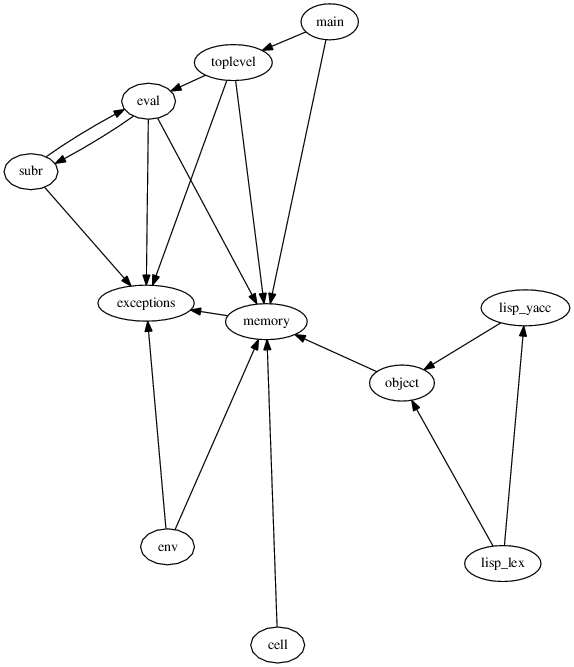
\includegraphics[scale=0.4]{graph.png}
    \label{fig:dep}
    \caption{Le graphe de dépendances de notre interpréteur}
  \end{center}
\end{figure}


On peut voir \textsc{Figure} \ref{fig:dep} le graphe de dépendances de notre interpréteur.

On constate que beaucoup de modules utilisent le module mémoire : que ce soit pour créer une mémoire dans \code{main}, le \code{toplevel} qui peut lancer le Garbage collector, ou les autres modules qui la manipulent.

De même, de nombreux modules sont susceptibles de lancer des exceptions.

\section{Mise en oeuvre et tests}

Pour vérifier le fonctionnement de la gestion mémoire, on rajoute une option (\code{-p}) qui affiche le statut du vecteur mémoire.

On parcourt le vecteur, et on affiche O si la case est occupée, et \_ sinon.

On peut ainsi facilement vérifier le fonctionnement du Garbage Collector.

Voici donc un exemple d'éxécution, avec une taille de mémoire initiale de 15, et un appel de Garbage Collector toutes les 30 allocations.

\lstset{language=C++,basicstyle=\ttfamily,breaklines=true, frame=single}
\begin{lstlisting}
  $ ./lisp -p
Creating Memory
Mem size : 15
Lisp Interpreter
Aurele Barriere & Jeremy Thibault
Printing memory vector
Lisp? (setq a 1)
OOOOOOOOO_____
Lisp? (- 6 5)
1
OOOOOOOOOOOOOOOOOOOOO________
Lisp? (setq f (lambda (n) (+ n 1)))
OOOOOOOOOOOOOOOOOOOOOOOOOOOOOOOOOOOOOOOOOOOOOOOO___________
collecting garbage
____O____________________O_O_O_O_O_O_OOO_OOO_______________
Lisp? (+ 1 2)
3
OOOOOOOOOOOOO____________O_O_O_O_O_O_OOO_OOO_______________
Lisp? (exit)
\end{lstlisting}
\lstset{language=C++,basicstyle=\ttfamily,breaklines=true}

On observe donc le fonctionnement de la mémoire. Quand on appelle trop de fois la méthode \code{allocate()}, le veteur mémoire s'aggrandit.

Et après le passage du Garbage collector, il ne reste plus qu'un objet des 2 premières commandes (a), et quelques objets pour la fonction f.

Ensuite, les prochains objets sont assignés au début du vecteur.

\section{Conclusion}

Ce projet fut pour nous l'occasion de rassembler tout ce que nous avions appris sur le C++, le Lisp et les interpréteurs.

Pour la première fois, nous avons pu nous intéresser de près à la gestion de la mémoire grâce à l'extension Garbage Collctor.


Cependant, notre projet aurait pu être amélioré :

Dans un premier temps, nous aurions pu créer la classe \code{Object}.
En effet, dans notre implémentation, un objet est un entier, et il existe donc des opérations qui peuvent le modifier. On aurait pu remplacer ce type par une classe contenant un seul champ : l'entier (l'indice dans le vecteur de la mémoire), un constructeur et une méthode pour accéder à l'indice. Toutes les méthodes seraient privées, et on listeraient quelques fonctions et classes amies qui pourraient s'en servir. Ainsi, notre approche aurait été encore plus sécurisée.

Ensuite, il aurait été possible de factoriser certaines fonctions (notamment celles qui interagissent avec les objets), pour une meilleure organisation et pour simplifier la déclaration des amis de la classe \code{memory}.

Enfin, notre Garbage Collector aurait pu bénéficier d'un compactage. En effet, après son éxécution, les objets restant sont éparpillés dans la mémoire. À cause du principe de localité et pour pouvoir réduire la taille de la mémoire occupé (dans le cas, par exemple, d'un programme ayant besoin de beaucoup de mémoire à l'initialisation, puis très peu ensuite), il aurait été utile de les regrouper au début du vecteur. Cependant, il aurait aussi fallu modifier les objets déplacés, puisque de nombreux objets pointent vers d'autres (dans le cas des listes par exemple).

Malgré les possibles améliorations, notre interpréteur est déjà beaucoup plus complet que la version qui nous était fournie. L'interaction avec l'utilisateur est mieux gérée (on ne considère pas qu'il ne se trompe jamais, mais on rattrape les exceptions liées à ses erreurs), et la mémoire est totalement contrôlée. Le code lui-même a égalment été redécouper par endroits pour mieux l'organiser.

\end{document}
